\documentclass[12pt,letterpaper,onecolumn]{article}
\usepackage{graphicx}
\usepackage{minted}
\usemintedstyle{arduino}
\setminted[c]{linenos, frame=lines}
\usepackage{mathptmx}
\newcommand{\titlefont}{\fontfamily{ptm}\fontseries{b}\fontsize{16pt}{\baselineskip}\selectfont}
\newcommand{\authorfont}{\fontfamily{ptm}\fontseries{b}\fontsize{14pt}{\baselineskip}\selectfont}
\newcommand{\zwfont}{\fontfamily{ptm}\fontsize{12pt}{\baselineskip}\selectfont}
\newcommand{\codefont}{\fontfamily{phv}\fontsize{11pt}{\baselineskip}\selectfont}
\newcommand{\headfont}{\fontfamily{ptm}\fontseries{b}\fontsize{12pt}{\baselineskip}\selectfont}
\usepackage{geometry}
\geometry{left = 1.0in,right = 1.0in,top = 1.0in,bottom = 1.0in}
\title{\titlefont Report for Lab 2\vspace{300pt}}
\author{\authorfont Muhan Li\\ \authorfont Man Sun\\ \authorfont Mingxiao An}
\date{}
\usepackage{titlesec}
\titleformat*{\section}{\headfont}
\titleformat*{\subsection}{\headfont}
\usepackage{xcolor}


\begin{document}
	\maketitle
	\thispagestyle{empty}
	\vspace{40pt}
	\hfill \newline
	\textbf{Statement}: we promise that all of the work in this lab and report are finished by ourselves.\\
	\textbf{Sign}: Muhan Li, Man Sun, Mingxiao An.\\
	\newpage
	\tableofcontents
	\newpage
	\section{ABSTRACT}	
	%	The abstract should provide a brief overview of the report - one paragraph at most. 
	%	
	%	It should provide a summary of the main specific points for the introduction, the main tests and experiments, the results, and the conclusions. It is called an abstract because you can literally "abstract" sentences from the other sections. 
	%	
	%	Once again, this is not a narrative of your experiences as you executed the design.  The abstract should mirror (albeit in a very condensed way) the content of your report.	
		In this report, we will give a brief introduction on the purpose and tools used in the lab, a very detailed discussion of the lab. the testplan we will apply, the result of the lab as well as its analysis,
the errors we met when doing this lab and the analysis, and the summary and conclusions of the whole lab and report. We will also hard copy our code used in this lab to the Appendices.
	\section{INTRODUCTION}
	%	Brief introduction and overview of the purpose of the lab and of the methods and tools used - one to two paragraphs at most.
		This lab is the second lab of EE300. It has two main purposes. The first is to build a more complex design, a calculator, using some peripherals in lab 1. The second is to begin to learn the formal design process during the development cycle. This lab is not about learning how to build, but how to design, which is a key skill in software development.
	\section{DISCUSSION OF THE LAB}
	%	This section should include the following:
	%	
	%	Brief Design Specification - In this subsection you will textually describe your client's requirements.  What does he or she need in the project you are developing.  If you are incorporating extra features or capabilities, please describe them clearly in this section.
	%	
	%	Overall summary description of the module - 2-3 paragraphs maximum
	%	
	%	Specification of the public interface to the module
	%	
	%	Inputs
	%	Outputs
	%	Side effects - what outside variables did the module change
	%	
	%	Pseudo English description of algorithms, functions, or procedures
	%	Error handling
	%	
	%	Hardware Implementation
	%	
	%	Draw the schematic / logic diagram of how you connected the parts...switches, chips, LEDs etc.
	%	
	%	Use standard symbols for simple electronic parts and appropriately labeled boxes for larger parts. Should be a cleaned-up "picture" of what your breadboard and components actually look like
	%	
	%	Do not actually take a picture and submit this.
	%	
	%	Software Implementation
	%	
	%	What is your design????
	%	
	%	Present your design starting from a top level functional view and potentially block diagram or high level architecture. 
	%	
	%	Refine that view to present and explain each of the modules that comprise the major functional blocks. 
	%	
	%	Discuss the flow of control through the design. 
	%	
	%	Identify and discuss the specific modules you have implemented in your design. Explain your design choices.  
		\subsection{Brief Design Specification}
\subsubsection{Overall summary description of the module}
This module should function as a calculator and be designed by ourselves. The input should be received from the serial monitor on a PC connected to the Arduino board, and the output should be both displayed on the serial monitor and a LCD screen connected to the board. The input digits and symbols and result should be displayed on the LCD screen in a specified format. Also, data transfer between two Arduino boards should be reflected on the module design.

	\section{TESTPLAN}
	%	Overall summary of what needs to be tested to ensure that your design meets the original requirements, 2-3 paragraphs maximum unless specified otherwise   
		We will need to test the correctness of the calculation, if the calculator can output proper error information when the input is invalid, and the robustness for different kinds of invalid inputs.For phase 2, first, we will need to test all the cases required in phase 1. Apart from that, we will also need to test if the calculator makes the 1-digit number input as invalid.For phase 3, all tests in phase 2 must be repeated in this phase. Meanwhile, handling on the input of positive and negative sign is necessary in the test plan of this phase. In the test plan for two processors, we will need to test if the bytes are correctly transferred from the master processor to the slave processor as well as all the tests in phase 3.
	\section{PRESENTATION, DISCUSSION, AND ANALYSIS OF THE RESULTS}
	%	Based upon the execution of your design, present your results. Explain them and what was expected, and draw any conclusions (for example, did this prove your design worked).
	%	
	%	In addition to a detailed discussion and analysis of your project and your results, you must include all the answers to all questions raised in the lab.
		\paragraph{phase 1}
We input "1+1=", "!", "2\&", "3/0=", "4+4~" successively to the serial monitor after we run the project. The output result of the serial monitor is shown in figure[\ref{fig:test1}]. The output result on LCD is the same as expected.
\begin{figure}[!htbp]
	\centering
	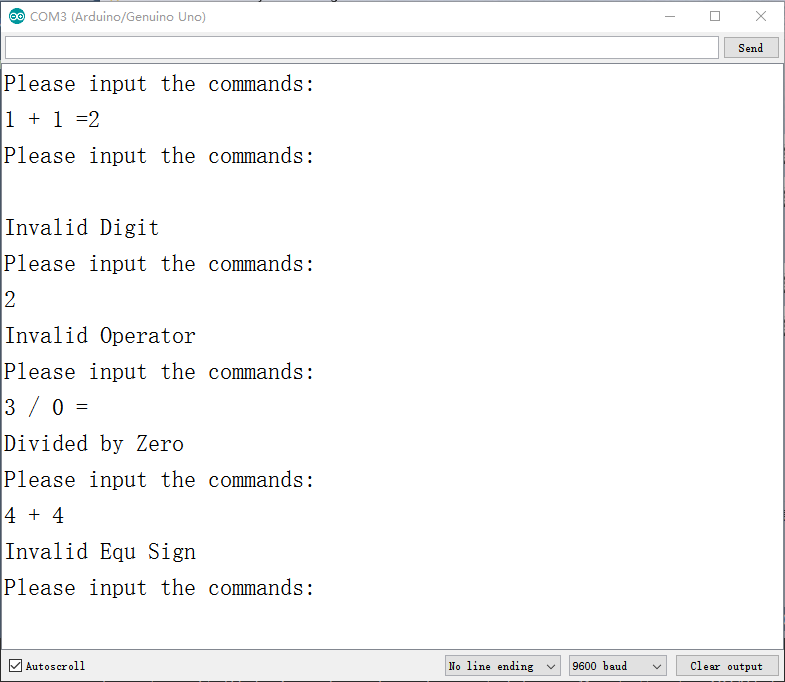
\includegraphics[width = \linewidth]{images/test1.png}
	\caption{Test result on serial monitor for phase 1}
	\label{fig:test1}
\end{figure}

\paragraph{phase 2}
We input "12+24=", "35*3", "34+!", "79\&", "67+90-", "87/00=" successively to the serial monitor after we run the project. The output result of the serial monitor is shown in figure[\ref{fig:test2}]. The output result on LCD is the same as expected.
\begin{figure}[!htbp]
	\centering
	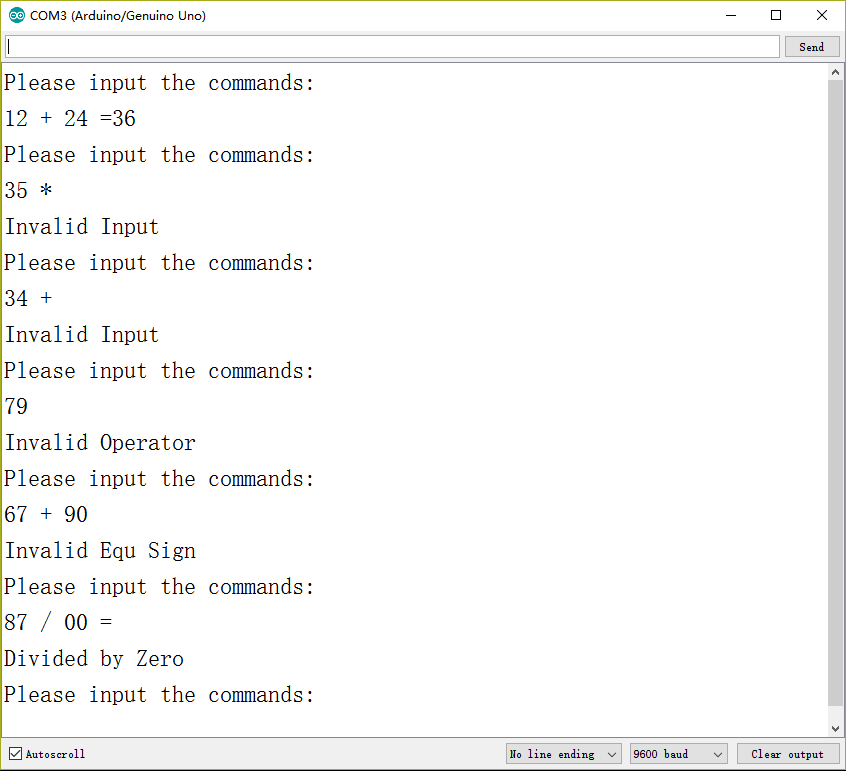
\includegraphics[width = \linewidth]{images/test2.png}
	\caption{Test result on serial monitor for phase 2}
	\label{fig:test2}
\end{figure}

\paragraph{phase 3}
We input "39-67=", "48(", "~", "28*45+", "90/00=", "-89*-23=", "78/-46=" successively to the serial monitor after we run the project. The output result of the serial monitor is shown in figure[\ref{fig:test3}]. The output result on LCD is the same as expected.
\begin{figure}[!htbp]
	\centering
	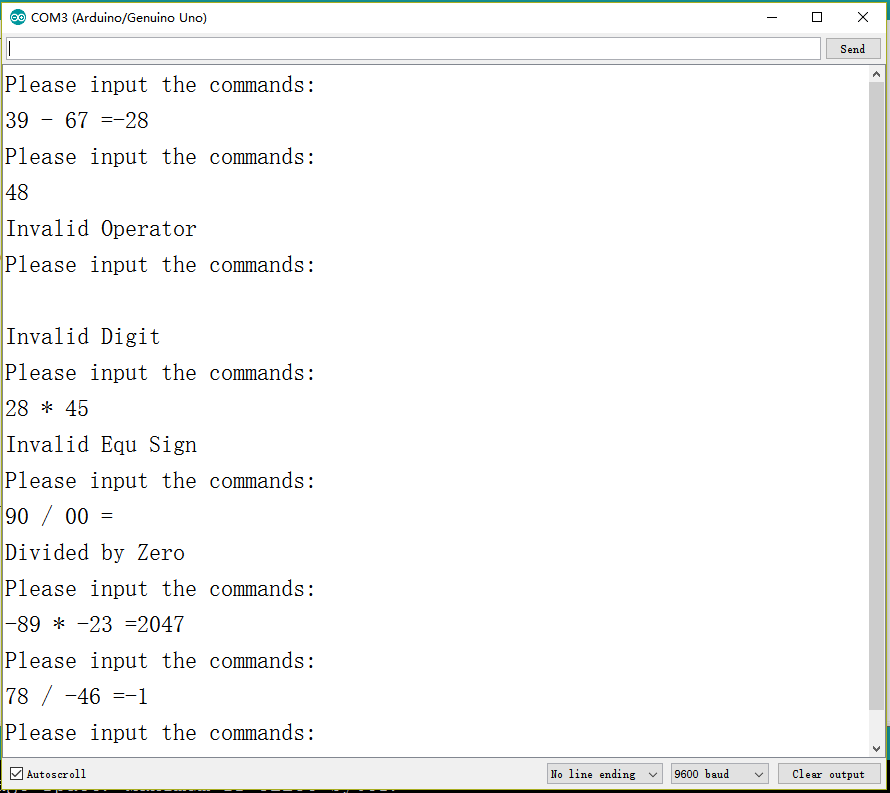
\includegraphics[width = \linewidth]{images/test3.png}
	\caption{Test result on serial monitor for phase 3}
	\label{fig:test3}
\end{figure}

\paragraph{two processors}
We input "12+29=", "42(", "3", "29*35+", "34/00=", "67+-38=" successively to the serial monitor of the master processor after we run the project on both processors. The output result of the serial monitor of the master and slave processors is shown in figure[\ref{fig:test4}]. The output result on LCD of the slave processor is the same as expected.
\begin{figure}[!htbp]
	\centering
	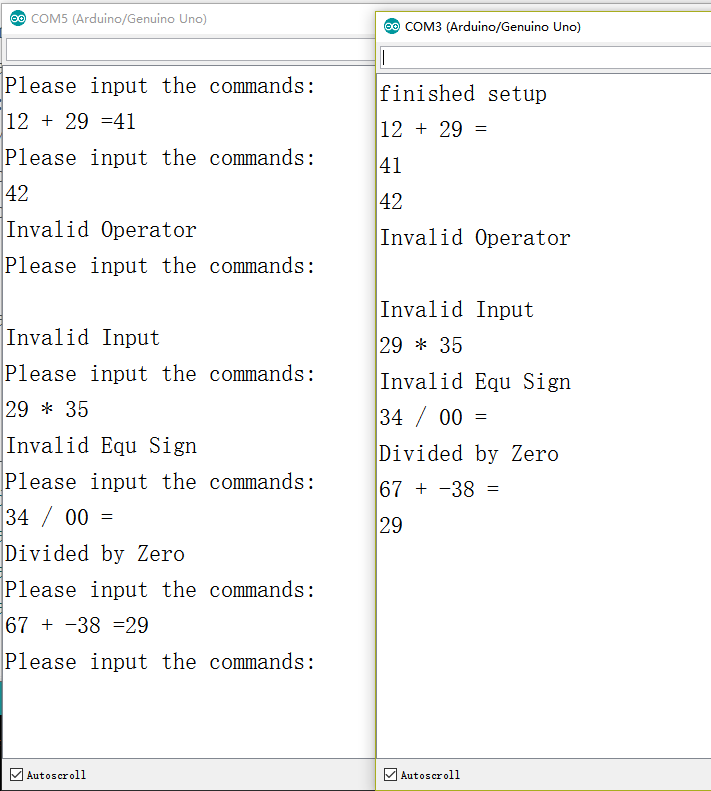
\includegraphics[width = \linewidth]{images/test4.png}
	\caption{Test result on serial monitor for phase 4}
	\label{fig:test4}
\end{figure}

	\section{ANALYSIS OF ANY ERRORS}
	%	This one is obvious. Do this section as appropriate.  If it improves the flow, it does not need to be a separate section and may be included in the presentation, discussion, and analysis of the results.  However, it will still be graded separately and must be present.
		When we are doing the lab with two processors, we connected the LCD to BUS3 on the slave board, which made the communication between two boards invalid. We could not receive anything from the master processor or send anything to the slave processor. When we pulled the connection off, we found that the communication worked on the serial monitors without LCD. 
%	\section{ANALYSIS OF WHY THE PROJECT MAY NOT OF WORKED AND WHAT EFFORTS WERE MADE TO IDENTIFY THE ROOT CAUSE OF ANY PROBLEMS}
%	%	State any problems you encountered while working on the project. If your project did not work or worked only partially, provide an analysis of why and what efforts were made to identify the root cause of any problems. Should be written only if your project (or a required component) did not work. 
%		\input{probs}
	\section{SUMMARY AND CONCLUSIONS}
	%	You should know these sections very well, no need to explain.  Note, however, that they are two different sections.  The summary is just that, a summary of your project.  It should loosely mirror the abstract with a bit more detail.  The conclusion concludes the report, potentially adds information that is often outside the main thrust of the report, and may offer suggestions or recommendations about the project.
		\paragraph{summary} In this report, we give a brief introduction on the purpose of the lab, a very detailed discussion of the lab. the testplan we will apply, the result of the lab as well as its
analysis, the errors we met when doing this lab and the analysis, and the summary and conclusions of the whole lab and report. We will also hard copy our code used in this lab to the Appendices.

\paragraph{conclusions} We successfully designed and implemented a calculator. We also became familiar with the formal design process.

	\section{APPENDICES}
	%	Your final version of any and all pseudocode and C code should go in this section. 
		\subsection{calculator.ino}
\begin{minted}{c}
//----------------------------------------------------------------
// Module name:
//    calculator.ino
// Languange:
//    Wiring/Arduino
// Description:
//    The program takes user's input from the Serial Monitor and
//	  prints the input and result on a LCD.
// Author:
//	  Mingxiao An, Man Sun, Muhan Li
//	Rev.0 12 July 2017
//  Rev.1 13 July 2017
//  Rev.2 16 July 2017
//----------------------------------------------------------------
#include "Arduino.h"
#include "headers/constant.h"
#include "headers/phase.h"
#include "headers/test.h"

#if PHASE == 0					// used for testing

// the setup routine runs once when you press reset:
void setup() {
    Serial.begin(BAUD_RATE);	// start serial port at baud rate
    test::setup();			  // use the setup function in test namespace
}

// the loop routine runs over and over again forever:
void loop() {
    test::loop();				// use the loop function in test namespace
}

#else							// used for displaying

// the setup routine runs once when you press reset:
void setup() {
    Serial.begin(BAUD_RATE);	// start serial port at baud rate
    phase::setup();				// use the setup function in test namespace
}

// the loop routine runs over and over again forever:
void loop() {
    phase::loop();				// use the loop function in test namespace
}

#endif	// PHASE == 0

\end{minted}
		
\end{document}